\documentclass[UTF8,zihao=-4,fontset=none]{ctexart}

\usepackage[a4paper,left=25mm,right=25mm,top=27mm,bottom=24mm,headheight=24pt]{geometry}
\usepackage{fontspec}
\usepackage{xeCJK}
\usepackage{amsmath,amssymb}
\usepackage{graphicx}
\usepackage{xcolor}
\usepackage{booktabs,tabularx,array,longtable,multirow}
\usepackage{caption}
\usepackage{enumitem}
\usepackage{setspace}
\usepackage{fancyhdr}
\usepackage{titlesec}
\usepackage{tikz}
\usepackage{microtype}
\usepackage{csquotes}
\usepackage{xurl}
\usepackage{hyperref}
\usepackage[nameinlink,noabbrev]{cleveref}
\usepackage[backend=biber,style=gb7714-2015,sorting=none,gbnamefmt=lowercase]{biblatex}
\usepackage[most]{tcolorbox}
\usepackage{placeins}
\usepackage{needspace}

\ifdefined\XeTeXgenerateactualtext
  \XeTeXgenerateactualtext=1
\fi

\usetikzlibrary{arrows.meta,positioning,fit,calc}
\addbibresource{references.bib}
\renewcommand*{\bibfont}{\footnotesize\setstretch{1.08}}

\setmainfont{texgyretermes-regular.otf}[
  BoldFont=texgyretermes-bold.otf,
  ItalicFont=texgyretermes-italic.otf,
  BoldItalicFont=texgyretermes-bolditalic.otf
]
\setsansfont{texgyreheros-regular.otf}[
  BoldFont=texgyreheros-bold.otf,
  ItalicFont=texgyreheros-italic.otf,
  BoldItalicFont=texgyreheros-bolditalic.otf
]
\setmonofont{lmmono10-regular.otf}
\setCJKmainfont{Songti SC}[AutoFakeBold=2.2]
\setCJKsansfont{PingFang SC}[AutoFakeBold=2.2]
\setCJKmonofont{STFangsong}

\definecolor{Ink}{HTML}{2D3436}
\definecolor{JinmenBlue}{HTML}{244C66}
\definecolor{BrickGrey}{HTML}{A8B0AB}
\definecolor{Cinnabar}{HTML}{A54432}
\definecolor{PaleJade}{HTML}{E9EFEA}
\definecolor{RicePaper}{HTML}{F7F3E8}
\definecolor{LightRule}{HTML}{D8DDD9}

\color{Ink}
\linespread{1.36}
\setlength{\parindent}{2em}
\setlength{\parskip}{0pt}
\setlength{\emergencystretch}{2em}
\setlist{nosep,leftmargin=2.2em,labelsep=.6em}
\setlist[itemize]{label=\textcolor{JinmenBlue}{\small\textbullet}}
\setlist[enumerate]{label=\textcolor{JinmenBlue}{\arabic*.}}

\titleformat{\section}
  {\Large\bfseries\sffamily\color{JinmenBlue}}
  {\thesection}{0.75em}{}
  [\vspace{0.2em}\color{LightRule}\titlerule]
\titleformat{\subsection}
  {\large\bfseries\sffamily\color{Ink}}
  {\thesubsection}{0.7em}{}
\titleformat{\subsubsection}
  {\normalsize\bfseries\sffamily\color{Ink}}
  {\thesubsubsection}{0.6em}{}
\titlespacing*{\section}{0pt}{2.7ex plus .5ex}{1.5ex}
\titlespacing*{\subsection}{0pt}{2.0ex plus .4ex}{.8ex}
\titlespacing*{\subsubsection}{0pt}{1.5ex}{.5ex}

\captionsetup{
  font=small,
  labelfont={bf,color=JinmenBlue},
  textfont={color=Ink},
  skip=6pt
}
\newcolumntype{Y}{>{\raggedright\arraybackslash}X}
\newcolumntype{P}[1]{>{\raggedright\arraybackslash}p{#1}}
\newcolumntype{C}[1]{>{\centering\arraybackslash}p{#1}}
\renewcommand{\arraystretch}{1.25}
\setlength{\tabcolsep}{5pt}

\hypersetup{
  colorlinks=true,
  linkcolor=JinmenBlue,
  citecolor=JinmenBlue,
  urlcolor=Cinnabar,
  pdfauthor={晏妍、王彦翔},
  pdftitle={海河少女：基于可信 RAG 的天津文化 AI 虚拟主播系统设计与实现},
  pdfsubject={天津文化 IP 主题 AI 虚拟主播系统},
  pdfkeywords={可信 RAG, 虚拟主播, 天津文化, VRM, 证据门控}
}
\crefname{figure}{图}{图}
\crefname{table}{表}{表}
\crefname{equation}{式}{式}

\pagestyle{fancy}
\fancyhf{}
\fancyhead[L]{\small\sffamily\color{BrickGrey} 天津师范大学}
\fancyhead[R]{\small\sffamily\color{BrickGrey} 系统设计与实现}
\fancyfoot[C]{\small\sffamily\color{BrickGrey}\thepage}
\renewcommand{\headrulewidth}{0.4pt}
\renewcommand{\headrule}{\hbox to\headwidth{\color{LightRule}\leaders\hrule height \headrulewidth\hfill}}
\renewcommand{\footrulewidth}{0pt}

\newtcolorbox{boundarybox}{
  enhanced,
  breakable,
  colback=PaleJade!45,
  colframe=JinmenBlue,
  boxrule=0pt,
  borderline west={2.2pt}{0pt}{JinmenBlue},
  arc=0pt,
  left=9pt,right=9pt,top=8pt,bottom=8pt,
  before skip=10pt,after skip=10pt
}

\newcommand{\keyword}[1]{\noindent\textbf{关键词：}#1}
\newcommand{\enkeyword}[1]{\noindent\textbf{Keywords: }#1}
\newcommand{\code}[1]{\texttt{#1}}
\newcommand{\yes}{\textcolor{JinmenBlue}{已验证}}
\newcommand{\pending}{\textcolor{Cinnabar}{待核验}}

\begin{document}

\hypersetup{pageanchor=false}
\pagecolor{RicePaper}
\begin{titlepage}
  \thispagestyle{empty}
  
\begin{tikzpicture}[remember picture,overlay]
    \fill[JinmenBlue] ([xshift=21mm]current page.north west) rectangle
      ([xshift=24mm]current page.south west);
    \draw[BrickGrey,line width=.5pt]
      ([xshift=31mm,yshift=-25mm]current page.north west) --
      ([xshift=-24mm,yshift=-25mm]current page.north east);
  \end{tikzpicture}

  \vspace*{17mm}
  {\sffamily\color{JinmenBlue}\large
    2026 年第十三届天津市大学生动漫与数字创意设计大赛\par}
  \vspace{3mm}
  {\sffamily\color{BrickGrey}\normalsize
    AI 虚拟主播赛道 · 天津文化 IP 主题\par}

  \vfill
  {\fontsize{34}{46}\selectfont\bfseries\sffamily\color{Ink}
    海河少女\par}
  \vspace{8mm}
  {\fontsize{20}{31}\selectfont\sffamily\color{JinmenBlue}
    基于可信 RAG 的天津文化\par
    AI 虚拟主播系统设计与实现\par}
  \vspace{13mm}
  {\large\color{Ink}
    面向证据约束问答、三维文化向导与语音播报的本地系统\par}

  \vfill
  \begin{center}
    \renewcommand{\arraystretch}{1.6}
    \begin{tabular}{@{}>{\bfseries\sffamily\raggedleft\arraybackslash}p{30mm}@{\hspace{10mm}}>{\raggedright\arraybackslash}p{70mm}@{}}
      学校 & 天津师范大学 \\
      作者 & 晏妍、王彦翔 \\
      指导教师 & 王欣雨 \\
      完成日期 & 2026 年 9 月 \\
    \end{tabular}
  \end{center}
  \vspace{8mm}
\end{titlepage}
\pagecolor{white}

\clearpage
\hypersetup{pageanchor=true}
\pagenumbering{Roman}
\pagestyle{plain}
\phantomsection
\addcontentsline{toc}{section}{摘要}
\begin{center}
  {\zihao{3}\bfseries\sffamily\color{JinmenBlue} 摘\quad 要\par}
\end{center}
\vspace{2.2em}
非物质文化遗产数字传播不仅要求形象具有地域辨识度，也要求自动生成内容能够说明依据。本文设计并实现“海河少女”天津文化 AI 虚拟主播系统：以 VRM 三维角色作为文化向导，以人工审核的限定知识库作为事实边界，以 SQLite FTS5 与文本向量组成混合检索，并在生成前后设置主题检查、证据阈值、引用白名单、数字与日期一致性检查以及独立语义复核。只有通过校验的回答才获得一次性语音令牌，从而把知识证据、文本生成和语音播报连接为可检查的闭环。系统现有知识库包含 22 个来源、347 个知识块，覆盖角色设定、泥人张、风筝魏、海河文化和天津海棠。2026 年 9 月 13 日，使用百炼 1024 维生产向量完成固定 60 题评测：40 个库内问题全部在 Top-6 命中预标来源，20 个越界、歧义与提示词攻击问题全部被拒答；正式 API 连续问答 20/20 通过，其中 2 轮真实语音请求均返回 HTTP 200，后端 30 项测试全部通过。浏览器亦已加载新 VRM 并完成 1920×1080 交互检查。同日的百炼新加坡业务空间联调还验证了固定快照生成模型、Momo 非实时 HTTP 语音合成及新增风筝魏问题的完整问答播报链路。上述数据只证明当前测试集和联调样例下的工程表现，不等同于大语言模型理论上绝对不会产生幻觉。VRM 书面授权、署名和隐私字段仍需在 9 月 23 日提交前完成复核。

\vspace{1.5em}
\keyword{可信 RAG；虚拟主播；天津文化；VRM；证据门控；非遗数字化}

\clearpage
\phantomsection
\addcontentsline{toc}{section}{Abstract}
\begin{center}
  {\zihao{3}\bfseries\sffamily\color{JinmenBlue} ABSTRACT\par}
\end{center}
\vspace{2.2em}
\noindent Digital communication of intangible cultural heritage requires both a recognisable regional identity and traceable evidence for generated statements. This paper presents \emph{Haihe Girl}, an AI virtual-presenter system for Tianjin culture. A VRM character serves as the cultural guide, while a manually reviewed and domain-bounded knowledge base defines the factual scope. The backend combines SQLite FTS5 lexical retrieval with dense-vector retrieval, followed by topic screening, evidence thresholds, citation allow-list checks, numerical and date consistency checks, and a separate semantic verification pass. Only answers that pass all checks receive a one-time token for speech synthesis, thereby connecting evidence retrieval, text generation, citation display, and spoken delivery in an auditable pipeline.

The current corpus contains 22 sources and 347 chunks covering the character design, Tianjin Clay Figurine Zhang, Kite Wei, Haihe River culture, and Tianjin crabapple imagery. On 13 September 2026, a fixed 60-question evaluation using the 1024-dimensional production embedding passed all predefined checks: all 40 in-scope questions retrieved a labelled source within the top six results, and all 20 out-of-scope, ambiguous, and prompt-injection questions were rejected. The formal 20-round API test passed 20/20; two real speech requests returned HTTP 200, and all 30 backend tests passed. The supplied VRM was also loaded in a 1920×1080 browser session. Integration in an Alibaba Cloud Model Studio Singapore workspace further verified fixed-snapshot JSON generation, Momo non-real-time HTTP speech synthesis, and the complete query-to-audio path for a newly added Kite Wei question. These results describe the present test set and integration samples; they do not imply that a large language model is theoretically incapable of hallucination. Written VRM authorisation, attribution, and private metadata remain pending before submission.

\vspace{1.5em}
\enkeyword{trustworthy RAG; virtual presenter; Tianjin culture; VRM; evidence gating; digital heritage}

\clearpage
\phantomsection
\renewcommand{\contentsname}{目\quad 录}
\setcounter{tocdepth}{1}
\tableofcontents

\clearpage
\pagestyle{fancy}
\pagenumbering{arabic}
\setcounter{page}{1}

\section{引言}

虚拟数字人兼具可视形象、语言表达和交互能力，正在成为文化展示与公共叙事的新媒介\cite{li2025digitalhuman}。然而，将通用大语言模型直接接入文化讲解，会引入两个相互关联的问题：其一，模型可能把记忆、推断或过时信息写成确定事实；其二，虚拟主播以自然语音和拟人形象输出时，受众更难察觉回答依据不足。检索增强生成（Retrieval-Augmented Generation, RAG）能够在生成前提供外部证据\cite{lewis2020rag}，但“检索到文档”并不自动意味着“回答被文档支持”。如果缺少范围门控、引用约束和拒答机制，带有引用外观的回答仍可能包含无依据内容。

本项目面向天津文化 IP 主题 AI 虚拟主播赛道，构建一个本地运行、证据可追踪的文化问答原型。角色视觉以泥人张仕女彩塑的温润气韵、海河的水色和五大道海棠意象为主要线索，将高密度的风筝魏符号保留在独立道具层，避免在服装表面堆叠文化元素。该设计遵循符号提取与数字媒介转译的思路\cite{yuan2026symbol,shao2025kite}，但不会把参赛团队的拟人化世界观写成历史事实。

本文的工程贡献包括以下三点：
\begin{enumerate}
  \item 建立角色创作资料、学术资料和官方资料并行的来源体系，在数据层保留来源类型、页码、片段、网址与文件哈希；
  \item 设计从检索到播报的多级证据门控，回答的每个事实段必须绑定本轮候选中的有效知识块，未通过校验的文本不能进入 TTS；
  \item 用固定 60 题检索集、20 轮端到端 API 问答和后端测试记录系统边界，并把“没有足够依据”作为正常产品状态而非异常兜底。
\end{enumerate}

\section{问题定义与设计目标}

\subsection{使用场景与核心矛盾}

本作品面向竞赛演示和校园文化展示两类场景。用户以中文文字询问天津非遗、海河文化或角色设计，系统在本地审核语料中检索，展示答案和证据，再由三维角色播报。该场景的核心矛盾不是“能否生成一段流畅文字”，而是“拟人化表达如何不超过证据能力”。语气越自然，受众越容易将其当作权威讲解；因此产品必须在视觉吸引力和事实克制之间建立可验证的约束。

本文将一次查询记为 $q$，检索到的候选知识块集合记为 $C_q$，生成回答的事实段集合记为 $P_q$。系统需要保证：每个 $p\in P_q$ 所声明的引用都来自 $C_q$，段落中的关键数字和日期能在证据中找到，并且语义复核判定证据能支持该段。若任一条件不成立，系统应返回拒答而不是补写看似合理的内容。

\subsection{功能、可信与展示目标}

\begin{table}[htbp]
\centering
\caption{系统目标与可验收出口}
\label{tab:goals}
\begin{tabularx}{\linewidth}{@{}P{28mm}Y Y@{}}
\toprule
目标类别 & 工程定义 & 验收出口 \\
\midrule
事实可追溯 & 每个事实段绑定服务端白名单内的知识块 & 前端可展开标题、页码、摘录与 URL \\
证据不足拒答 & 越界、实时、歧义或低相关度问题不进入生成 & 返回固定拒答，无引用、无语音令牌 \\
播报权限隔离 & 前端不能把任意文本直接交给 TTS & 仅已校验回答获得一次性令牌 \\
三维交互稳定 & 模型、字幕、引用和音频状态不相互遮挡 & 1920\texttimes1080 下连续问答无崩溃 \\
材料可复现 & 源码、配置示例、评测集和论文保持一致 & 无密钥、索引元数据匹配、PDF 可完整解析 \\
\bottomrule
\end{tabularx}
\end{table}

\subsection{明确非目标}

为在 9 月 23 日前交付一条可靠主链，项目不建设公网服务，不开放用户上传文档，不在运行时联网搜索，不接入麦克风语音识别，也不在云服务失败时播放预录音频冒充实时回答。这些限制使系统能够对资料范围、版本和错误状态做出明确说明。“不瞎编”因而是一个由数据治理、证据门控和固定评测共同支撑的工程目标，而非对模型本体的绝对能力声明。

\section{文化 IP 与视觉转译}

\subsection{角色定位与来源边界}

“海河少女”被设定为了解天津手工艺与海河城市文化的年轻讲述者。泥人张和彩塑相关事实优先依据国家级非物质文化遗产项目资料\cite{ihchinaNiren}；风筝魏的项目身份与技艺信息依据国家级非遗公开资料\cite{ihchinaKite}；海河和海棠作为城市意象时，分别依据天津市文化和旅游局资料\cite{tianjinHaihe,tianjinBegonia}。角色“常驻海河、随潮汐收集城市记忆”等描述是作品世界观，只能在创作设定语境中使用。

知识库为两类信息设置了不同标签。历史、名录、技艺和城市资料标记为 \code{factual}，角色性格、服装转译和故事背景标记为 \code{creative}。当问题询问角色外观或世界观时，系统优先召回团队原创设定；当问题涉及历史事实时，创作资料不能代替官方或学术来源。该分离减少了叙事语言与史实陈述之间的混淆。

\subsection{造型、色彩与制作过程}

角色上衣以低饱和深青为主，裙摆使用柔粉和白色窄边，朱红系带仅承担点睛作用；黑蓝渐变发色将海河水色转化为不依赖具象图案的视觉线索。服装保持交领、束腰和分层裙摆的结构感，同时减少大面积纹样。角色主体现代、简洁，风筝符号承担更高的信息密度，从而形成“主体克制、道具强调”的层次。

\begin{figure}[htbp]
  \centering
  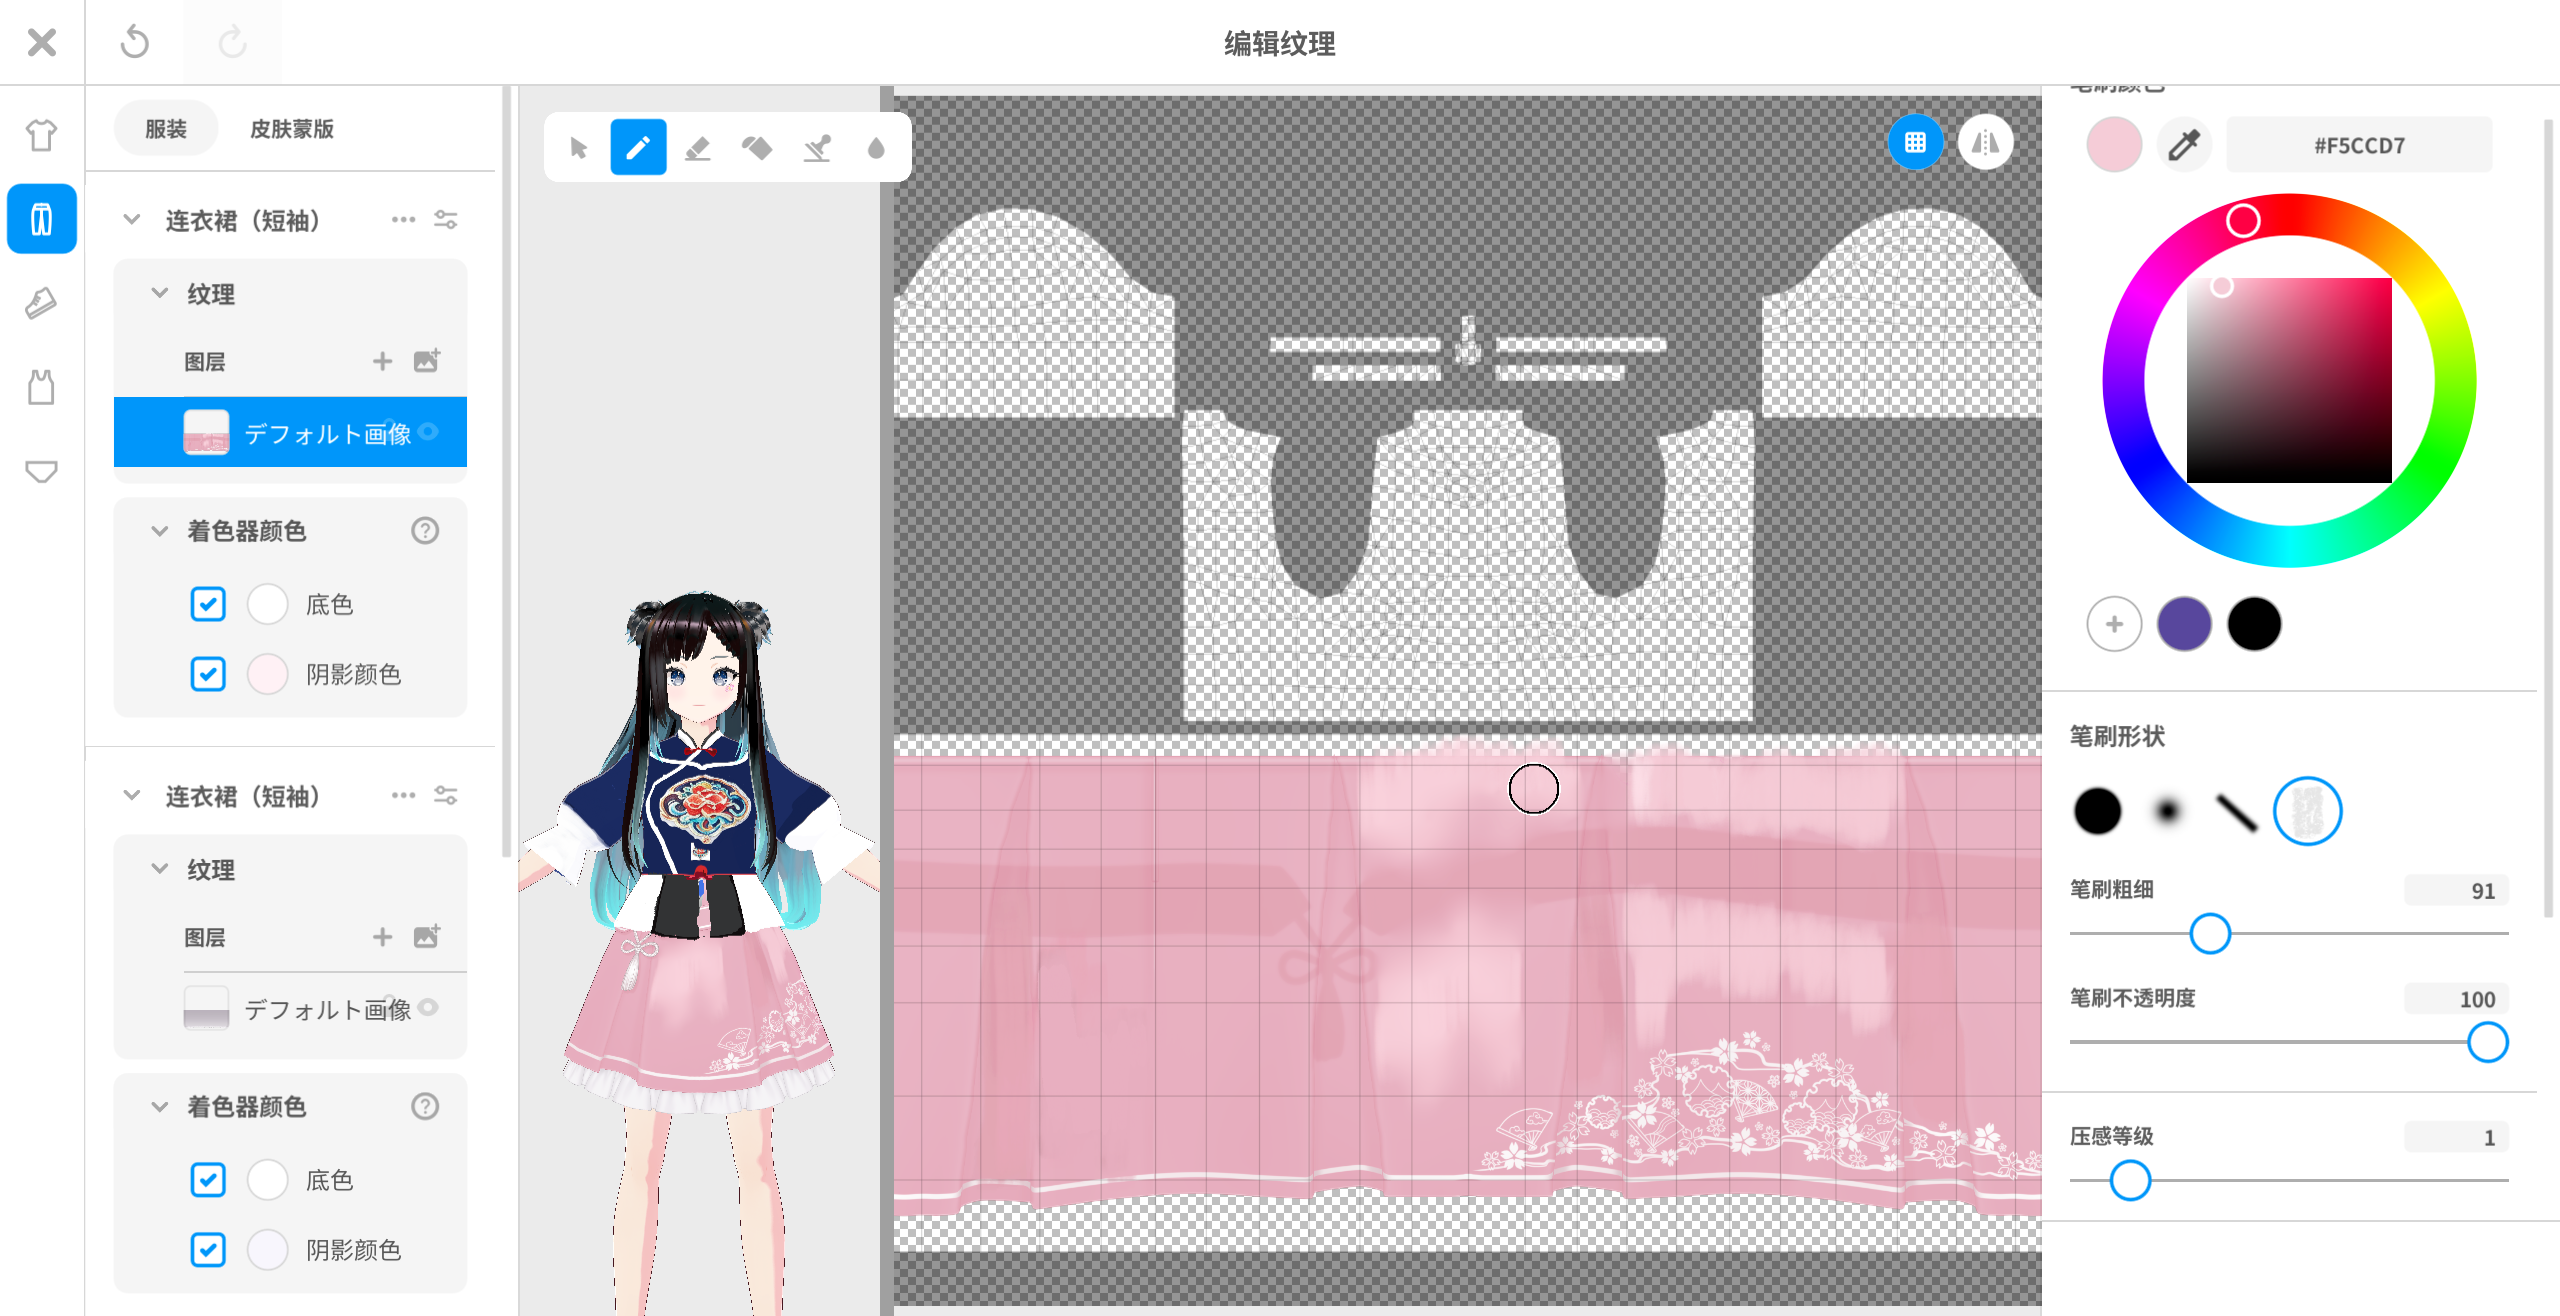
\includegraphics[width=.9\linewidth]{../海河少女/人物设计过程/3cdfb743e2d76f972399badb1bd1d1c1.png}
  \caption{海河少女裙摆纹理与色彩调整界面}
  \label{fig:vroid-skirt}
\end{figure}

\begin{figure}[htbp]
  \centering
  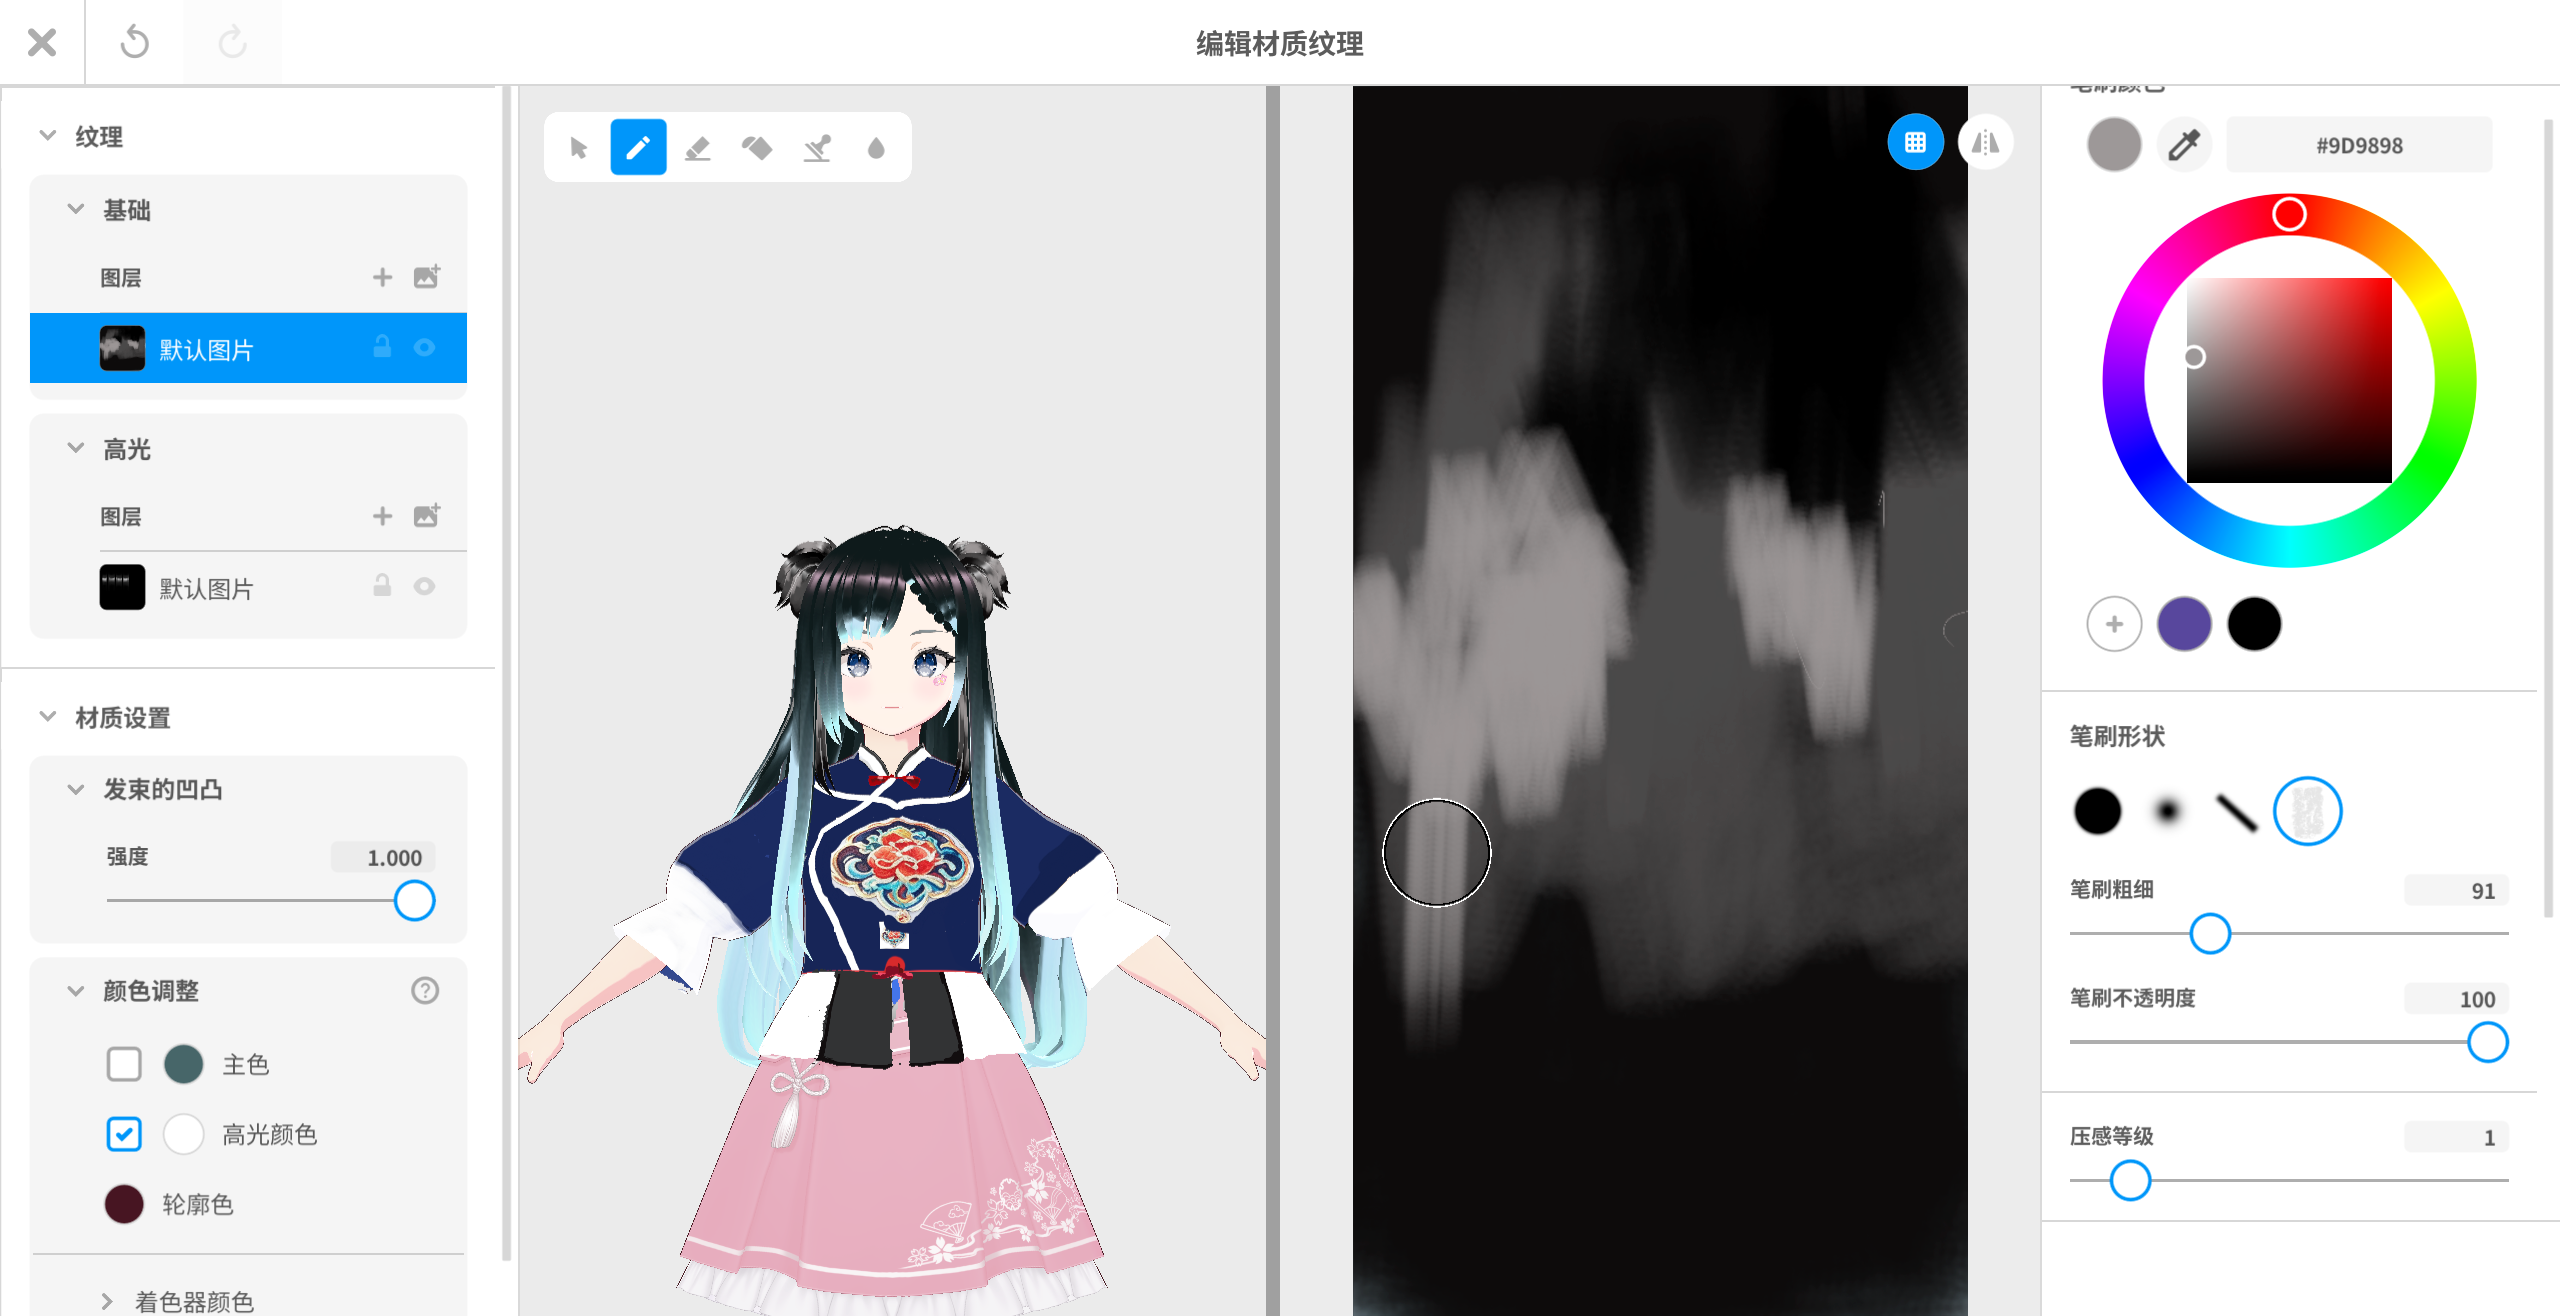
\includegraphics[width=.9\linewidth]{../海河少女/人物设计过程/8fc0881b93edd0a068ebc5579a076749.png}
  \caption{海河少女发色材质与高光调整界面}
  \label{fig:vroid-hair}
\end{figure}

图~\ref{fig:vroid-skirt} 和图~\ref{fig:vroid-hair}记录的是创作过程，而非自动生成的最终宣传图。论文不使用来源不明、带有第三方平台水印的造型参考图；相关参考只在能够确认作者、用途和许可时进入最终参赛材料。

\FloatBarrier

\section{系统架构}

\subsection{组件与数据边界}

系统由知识入库、检索与生成后端、三维交互前端和云端语音服务四部分组成。前端采用 React、TypeScript、Three.js 与 \code{@pixiv/three-vrm}\cite{threevrm}；后端采用 FastAPI，通过 Server-Sent Events（SSE）返回检索、校验、生成片段和最终引用。浏览器仅接收已经经过后端校验的数据，不能自行构造可播报文本。

\begin{figure}[htbp]
  \centering
  % 海河少女系统架构图
% 接口：主文已定义 Ink、JinmenBlue、BrickGrey、Cinnabar、PaleJade、RicePaper。
% 在 figure 环境中直接使用 % 海河少女系统架构图
% 接口：主文已定义 Ink、JinmenBlue、BrickGrey、Cinnabar、PaleJade、RicePaper。
% 在 figure 环境中直接使用 % 海河少女系统架构图
% 接口：主文已定义 Ink、JinmenBlue、BrickGrey、Cinnabar、PaleJade、RicePaper。
% 在 figure 环境中直接使用 \input{figures/system-architecture}。
\begin{tikzpicture}[x=1mm,y=1mm]
  \path[use as bounding box] (0,0) rectangle (158,60);

  \tikzset{
    hhArchBase/.style={
      draw=BrickGrey,
      fill=white,
      line width=.55pt,
      rounded corners=1.2mm,
      minimum width=31mm,
      minimum height=14mm,
      text width=27mm,
      inner sep=1.5mm,
      align=center,
      font=\small\sffamily,
      text=Ink
    },
    hhArchCore/.style={
      hhArchBase,
      draw=JinmenBlue,
      line width=.8pt,
      fill=PaleJade!62
    },
    hhArchGuard/.style={
      hhArchBase,
      draw=Cinnabar,
      line width=.8pt,
      fill=RicePaper
    },
    hhArchFlow/.style={
      -{Latex[length=2.1mm,width=1.45mm]},
      draw=JinmenBlue,
      line width=.75pt,
      line cap=round,
      line join=round
    },
    hhArchReject/.style={
      -{Latex[length=2.1mm,width=1.45mm]},
      draw=Cinnabar,
      line width=.75pt,
      line cap=round,
      line join=round
    }
  }

  % 上层：从受控来源到带引用的结构化回答。
  \node[hhArchBase]  (source) at (16,50)
    {\textbf{审核来源}\\[-.2ex]\scriptsize PDF\,/\,DOCX\,/\,MD};
  \node[hhArchCore]  (index)  at (57,50)
    {\textbf{混合索引}\\[-.2ex]\footnotesize FTS5 + 向量};
  \node[hhArchGuard] (gate)   at (98,50)
    {\textbf{证据门控}\\[-.2ex]\footnotesize 范围・阈值・来源};
  \node[hhArchCore]  (gen)    at (139,50)
    {\textbf{结构化生成}\\[-.2ex]\footnotesize 事实段绑定引用};

  % 下层反向回流：复核、授权、流式传输与数字人呈现。
  \node[hhArchBase] (front)  at (16,8)
    {\textbf{文化向导}\\[-.2ex]\footnotesize React + VRM};
  \node[hhArchCore] (sse)    at (57,8)
    {\textbf{流式传输}\\[-.2ex]\footnotesize 字幕・引用・状态};
  \node[hhArchCore] (token)  at (98,8)
    {\textbf{播报授权}\\[-.2ex]\footnotesize 一次性语音令牌};
  \node[hhArchGuard] (verify) at (139,8)
    {\textbf{回答复核}\\[-.2ex]\footnotesize 引用・数字・语义};

  \draw[hhArchFlow] (source.east) -- (index.west);
  \draw[hhArchFlow] (index.east)  -- (gate.west);
  \draw[hhArchFlow] (gate.east)   -- (gen.west);
  \draw[hhArchFlow] (gen.south)   -- (verify.north);
  \draw[hhArchFlow] (verify.west) -- (token.east);
  \draw[hhArchFlow] (token.west)  -- (sse.east);
  \draw[hhArchFlow] (sse.west)    -- (front.east);

  % 证据不足时不进入生成与语音授权，但仍经 SSE 向前端返回可见状态。
  \node[hhArchGuard,minimum width=27mm,minimum height=11mm,text width=23mm]
    (reject) at (98,29) {\textbf{固定拒答}\\[-.2ex]\footnotesize 不进入 TTS};
  \draw[hhArchReject] (gate.south) -- (reject.north);
  \draw[hhArchReject] (reject.west) -- ++(-8mm,0) -| (sse.north);
\end{tikzpicture}
。
\begin{tikzpicture}[x=1mm,y=1mm]
  \path[use as bounding box] (0,0) rectangle (158,60);

  \tikzset{
    hhArchBase/.style={
      draw=BrickGrey,
      fill=white,
      line width=.55pt,
      rounded corners=1.2mm,
      minimum width=31mm,
      minimum height=14mm,
      text width=27mm,
      inner sep=1.5mm,
      align=center,
      font=\small\sffamily,
      text=Ink
    },
    hhArchCore/.style={
      hhArchBase,
      draw=JinmenBlue,
      line width=.8pt,
      fill=PaleJade!62
    },
    hhArchGuard/.style={
      hhArchBase,
      draw=Cinnabar,
      line width=.8pt,
      fill=RicePaper
    },
    hhArchFlow/.style={
      -{Latex[length=2.1mm,width=1.45mm]},
      draw=JinmenBlue,
      line width=.75pt,
      line cap=round,
      line join=round
    },
    hhArchReject/.style={
      -{Latex[length=2.1mm,width=1.45mm]},
      draw=Cinnabar,
      line width=.75pt,
      line cap=round,
      line join=round
    }
  }

  % 上层：从受控来源到带引用的结构化回答。
  \node[hhArchBase]  (source) at (16,50)
    {\textbf{审核来源}\\[-.2ex]\scriptsize PDF\,/\,DOCX\,/\,MD};
  \node[hhArchCore]  (index)  at (57,50)
    {\textbf{混合索引}\\[-.2ex]\footnotesize FTS5 + 向量};
  \node[hhArchGuard] (gate)   at (98,50)
    {\textbf{证据门控}\\[-.2ex]\footnotesize 范围・阈值・来源};
  \node[hhArchCore]  (gen)    at (139,50)
    {\textbf{结构化生成}\\[-.2ex]\footnotesize 事实段绑定引用};

  % 下层反向回流：复核、授权、流式传输与数字人呈现。
  \node[hhArchBase] (front)  at (16,8)
    {\textbf{文化向导}\\[-.2ex]\footnotesize React + VRM};
  \node[hhArchCore] (sse)    at (57,8)
    {\textbf{流式传输}\\[-.2ex]\footnotesize 字幕・引用・状态};
  \node[hhArchCore] (token)  at (98,8)
    {\textbf{播报授权}\\[-.2ex]\footnotesize 一次性语音令牌};
  \node[hhArchGuard] (verify) at (139,8)
    {\textbf{回答复核}\\[-.2ex]\footnotesize 引用・数字・语义};

  \draw[hhArchFlow] (source.east) -- (index.west);
  \draw[hhArchFlow] (index.east)  -- (gate.west);
  \draw[hhArchFlow] (gate.east)   -- (gen.west);
  \draw[hhArchFlow] (gen.south)   -- (verify.north);
  \draw[hhArchFlow] (verify.west) -- (token.east);
  \draw[hhArchFlow] (token.west)  -- (sse.east);
  \draw[hhArchFlow] (sse.west)    -- (front.east);

  % 证据不足时不进入生成与语音授权，但仍经 SSE 向前端返回可见状态。
  \node[hhArchGuard,minimum width=27mm,minimum height=11mm,text width=23mm]
    (reject) at (98,29) {\textbf{固定拒答}\\[-.2ex]\footnotesize 不进入 TTS};
  \draw[hhArchReject] (gate.south) -- (reject.north);
  \draw[hhArchReject] (reject.west) -- ++(-8mm,0) -| (sse.north);
\end{tikzpicture}
。
\begin{tikzpicture}[x=1mm,y=1mm]
  \path[use as bounding box] (0,0) rectangle (158,60);

  \tikzset{
    hhArchBase/.style={
      draw=BrickGrey,
      fill=white,
      line width=.55pt,
      rounded corners=1.2mm,
      minimum width=31mm,
      minimum height=14mm,
      text width=27mm,
      inner sep=1.5mm,
      align=center,
      font=\small\sffamily,
      text=Ink
    },
    hhArchCore/.style={
      hhArchBase,
      draw=JinmenBlue,
      line width=.8pt,
      fill=PaleJade!62
    },
    hhArchGuard/.style={
      hhArchBase,
      draw=Cinnabar,
      line width=.8pt,
      fill=RicePaper
    },
    hhArchFlow/.style={
      -{Latex[length=2.1mm,width=1.45mm]},
      draw=JinmenBlue,
      line width=.75pt,
      line cap=round,
      line join=round
    },
    hhArchReject/.style={
      -{Latex[length=2.1mm,width=1.45mm]},
      draw=Cinnabar,
      line width=.75pt,
      line cap=round,
      line join=round
    }
  }

  % 上层：从受控来源到带引用的结构化回答。
  \node[hhArchBase]  (source) at (16,50)
    {\textbf{审核来源}\\[-.2ex]\scriptsize PDF\,/\,DOCX\,/\,MD};
  \node[hhArchCore]  (index)  at (57,50)
    {\textbf{混合索引}\\[-.2ex]\footnotesize FTS5 + 向量};
  \node[hhArchGuard] (gate)   at (98,50)
    {\textbf{证据门控}\\[-.2ex]\footnotesize 范围・阈值・来源};
  \node[hhArchCore]  (gen)    at (139,50)
    {\textbf{结构化生成}\\[-.2ex]\footnotesize 事实段绑定引用};

  % 下层反向回流：复核、授权、流式传输与数字人呈现。
  \node[hhArchBase] (front)  at (16,8)
    {\textbf{文化向导}\\[-.2ex]\footnotesize React + VRM};
  \node[hhArchCore] (sse)    at (57,8)
    {\textbf{流式传输}\\[-.2ex]\footnotesize 字幕・引用・状态};
  \node[hhArchCore] (token)  at (98,8)
    {\textbf{播报授权}\\[-.2ex]\footnotesize 一次性语音令牌};
  \node[hhArchGuard] (verify) at (139,8)
    {\textbf{回答复核}\\[-.2ex]\footnotesize 引用・数字・语义};

  \draw[hhArchFlow] (source.east) -- (index.west);
  \draw[hhArchFlow] (index.east)  -- (gate.west);
  \draw[hhArchFlow] (gate.east)   -- (gen.west);
  \draw[hhArchFlow] (gen.south)   -- (verify.north);
  \draw[hhArchFlow] (verify.west) -- (token.east);
  \draw[hhArchFlow] (token.west)  -- (sse.east);
  \draw[hhArchFlow] (sse.west)    -- (front.east);

  % 证据不足时不进入生成与语音授权，但仍经 SSE 向前端返回可见状态。
  \node[hhArchGuard,minimum width=27mm,minimum height=11mm,text width=23mm]
    (reject) at (98,29) {\textbf{固定拒答}\\[-.2ex]\footnotesize 不进入 TTS};
  \draw[hhArchReject] (gate.south) -- (reject.north);
  \draw[hhArchReject] (reject.west) -- ++(-8mm,0) -| (sse.north);
\end{tikzpicture}

\caption{从审核来源到三维主播输出的系统数据流。红色路径表示不满足证据条件时跳过生成或播报。}
\label{fig:architecture}
\end{figure}

\subsection{信任边界与责任分层}

系统把“资料是否允许入库”、“候选证据是否足够”、“生成文本是否被引用支持”和“文本是否允许播报”分成四个决策点。资料准入由团队人工完成；检索器只能从登记语料中取得候选；生成模型只负责在候选内组织表达；服务端则使用确定性规则与独立语义检查收回最终决策权。前端和 TTS 都不被视为事实决策者。

\begin{table}[htbp]
\centering
\caption{组件的可信边界}
\label{tab:trust-boundary}
\begin{tabularx}{\linewidth}{@{}P{28mm}Y Y@{}}
\toprule
组件 & 允许行为 & 明确禁止 \\
\midrule
入库工具 & 读取登记文件、生成哈希、切块和索引 & 将未审核文档自动加入生产库 \\
检索器 & 返回词法和向量候选，执行主题与相关度门控 & 在向量服务失败时悄然降级为无约束生成 \\
生成模型 & 根据知识块 ID 输出结构化事实段 & 自行添加未检索的书目或引用 \\
后端校验器 & 重建引用、检查数字日期、签发语音令牌 & 将未通过的文本作为“部分可用”播报 \\
浏览器前端 & 展示 SSE 状态、最终回答和服务端引用 & 修改引用 ID 或直接提交任意 TTS 文本 \\
\bottomrule
\end{tabularx}
\end{table}

\subsection{接口设计}

\begin{table}[htbp]
\centering
\caption{主要接口及约束}
\label{tab:api}
\small
\begin{tabularx}{\linewidth}{@{}P{42mm}P{25mm}Y Y@{}}
\toprule
接口 & 主要输入 & 输出 & 约束 \\
\midrule
\code{GET /api/health} & 无 & 索引、模型、TTS、VRM 状态 & 不返回密钥 \\
\code{POST /api/query} & 问题、会话 ID & SSE 状态、证据、回答、引用或拒答 & 输入限长，先门控后生成 \\
\code{POST /api/speech} & 一次性语音令牌 & WAV 音频 & 令牌约 5 分钟有效且使用后失效 \\
\code{GET /api/sources/\{id\}} & 来源及知识块 ID & 本地来源片段或官方链接描述 & 仅访问登记来源 \\
\bottomrule
\end{tabularx}
\end{table}

回答引用对象包含 \code{source\_id}、\code{chunk\_id}、标题、发布者、页码、原文片段和 URL。前端展示的引用由服务端依据本轮检索结果重建，而非直接相信模型输出的书目文本。

\subsection{查询状态机与并发控制}

一次正常查询依次经过待机、检索、生成、复核和播报状态；拒答和错误是与成功回答并列的终止状态。SSE 会传输 \code{status}、\code{evidence}、\code{token}、\code{final} 或 \code{error} 事件，但只有 \code{final} 事件中的引用可视为最终结果。检索期间展示的候选证据只是过程信息，不得被前端提前标记为“已验证”。

前端为每次提问递增请求序号，并使用 \code{AbortController} 取消上一个未完成请求。每个流式事件在写入界面前都比对当前序号，从而避免慢请求在新问题之后回写旧答案。开始新问题时会同时停止旧音频、清空旧引用和令牌，使角色口型、字幕与当前问题保持一致。

\begin{figure}[htbp]
  \centering
  % 从提问到播报的前后端状态机
\begin{tikzpicture}[x=1mm,y=1mm]
  \path[use as bounding box] (0,0) rectangle (158,63);
  \tikzset{
    hhState/.style={
      draw=JinmenBlue, fill=PaleJade!52, line width=.72pt,
      rounded corners=1.2mm, minimum width=22mm, minimum height=14mm,
      text width=18.5mm, align=center, inner sep=1.1mm,
      font=\small\sffamily, text=Ink
    },
    hhStateGuard/.style={hhState,draw=Cinnabar,fill=RicePaper},
    hhStateFlow/.style={
      -{Latex[length=2mm,width=1.35mm]}, draw=JinmenBlue,
      line width=.72pt, line cap=round, line join=round
    },
    hhStateFail/.style={
      -{Latex[length=2mm,width=1.35mm]}, draw=Cinnabar,
      line width=.72pt, line cap=round, line join=round
    }
  }

  \node[hhState] (idle) at (11,48) {\textbf{待机}\\[-.2ex]\footnotesize 接收问题};
  \node[hhState] (retrieve) at (38,48) {\textbf{检索}\\[-.2ex]\footnotesize 候选证据};
  \node[hhStateGuard] (gate) at (65,48) {\textbf{证据门控}\\[-.2ex]\footnotesize 范围・相关度};
  \node[hhState] (generate) at (92,48) {\textbf{生成}\\[-.2ex]\footnotesize 事实段};
  \node[hhState] (verify) at (119,48) {\textbf{引用复核}\\[-.2ex]\footnotesize ID・数字・语义};
  \node[hhState] (speech) at (146,48) {\textbf{播报}\\[-.2ex]\footnotesize 一次性令牌};

  \node[hhStateGuard,minimum width=30mm,text width=26mm] (scopeRefuse) at (65,9)
    {\textbf{范围拒答}\\[-.2ex]\scriptsize 越界或证据不足};
  \node[hhStateGuard,minimum width=30mm,text width=26mm] (checkRefuse) at (119,9)
    {\textbf{校验拒答}\\[-.2ex]\scriptsize 引用或语义不通过};
  \node[hhStateGuard,minimum width=22mm,text width=18mm] (error) at (146,9)
    {\textbf{可见错误}\\[-.2ex]\scriptsize 不伪造结果};

  \draw[hhStateFlow] (idle.east) -- (retrieve.west);
  \draw[hhStateFlow] (retrieve.east) -- (gate.west);
  \draw[hhStateFlow] (gate.east) -- node[above,font=\tiny\sffamily,text=BrickGrey] {是} (generate.west);
  \draw[hhStateFlow] (generate.east) -- (verify.west);
  \draw[hhStateFlow] (verify.east) -- node[above,font=\tiny\sffamily,text=BrickGrey] {通过} (speech.west);

  % 两条拒答分支均垂直进入各自终止状态，不交叉、不共用轨道。
  \draw[hhStateFail] (gate.south) -- node[right,font=\tiny\sffamily,text=Cinnabar] {否} (scopeRefuse.north);
  \draw[hhStateFail] (verify.south) -- node[right,font=\tiny\sffamily,text=Cinnabar] {否} (checkRefuse.north);

  % 云端异常是任一云调用均可能触发的独立终止条件，不错误归属于某一步。
  \node[font=\tiny\sffamily,text=Cinnabar,align=center] (cloudFail) at (146,27)
    {任一云调用失败};
  \draw[hhStateFail] (cloudFail.south) -- (error.north);

  \node[font=\scriptsize\sffamily,text=BrickGrey,anchor=south]
    at (80,59) {SSE 仅用于传输当前服务端状态；新问题会取消旧请求};
\end{tikzpicture}

  \caption{查询、拒答、错误与播报的前后端状态机}
  \label{fig:query-state}
\end{figure}

\FloatBarrier

\section{可信 RAG 方法}

\subsection{知识治理与切块}

当前语料由 2 份团队原创角色文档、10 篇学术研究资料、4 份官方资料摘编和 6 份审核网页摘编组成。新增学术资料主要涉及风筝魏符号转译、文化基因图谱与海河流域水环境\cite{jiang2024kite,tianjinKiteWeiSheet,kiteGeneMap,tan2002haihe}；新增网页覆盖天津城市沿革、海河通识和泥人张背景\cite{zhihuTianjinGeography,zhihuTianjinCity,tjrdHistory,baiduHaihe,ihchinaNiren,vcgBasketLady,thepaperNirenzhang}。入库程序解析 PDF、DOCX 与 Markdown，在标题或页码范围内按约 400 个字符切块，相邻块保留约 80 个字符重叠。新增四份学术 PDF 为图像型扫描件，入库时使用按页人工复核的文本，同时保留原 PDF 哈希和页码。每个知识块继承来源 ID、标题、发布者、主题、页码、URL 与文件 SHA-256 哈希。学术论文只用于小段检索和页码引用，不随参赛包再次分发全文；知乎和百度百科摘编仅作辅助资料，官方页面与论文证据优先。

\begin{table}[htbp]
\centering
\caption{知识来源组成及使用边界}
\label{tab:corpus}
\begin{tabularx}{\linewidth}{@{}p{31mm}C{15mm}Y Y@{}}
\toprule
来源类型 & 数量 & 主要用途 & 使用边界 \\
\midrule
原创角色资料 & 2 & 外观、性格、世界观与创作方法 & 明确标记为创作设定 \\
学术资料 & 10 & 非遗研究、视觉转译与虚拟人设计 & 按页码引用，不公开全文 \\
官方资料摘编 & 4 & 项目身份、城市文化与活动事实 & 保留网址和核验日期 \\
审核网页摘编 & 6 & 城市历史、海河与泥人张背景 & 二级来源只作辅助 \\
\midrule
合计 & 22 & 347 个知识块 & 运行时不联网扩展 \\
\bottomrule
\end{tabularx}
\end{table}

\subsection{来源准入与可追溯入库}

知识库不接受运行时临时抓取。每个来源必须先在 \code{knowledge/sources.json} 登记唯一 ID、标题、发布者、主题、文件类型、本地路径或 URL，并填写用途与授权边界。入库工具仅遍历该清单；目录中存在但未登记的文件不会被默认吸收。此设计将“拿到文件”与“允许作为系统证据”明确分开。

原始 PDF 在解析前计算 SHA-256。对具有文本层的 PDF，系统保留页码结构后切块；对新增的图像型扫描件，OCR 只用于产生待校对初稿，最终入库文本按页人工复核。字序、专名、年份和“申报”与“入选”等语义差异优先核对，避免将 OCR 错字转化为系统事实。审核文本与原文件分开存放，引用仍指向原 PDF 的真实页码。

\begin{figure}[htbp]
  \centering
  % 审核语料的入库与溯源生命周期
\begin{tikzpicture}[x=1mm,y=1mm]
  \path[use as bounding box] (0,0) rectangle (158,63);
  \tikzset{
    hhSource/.style={
      draw=JinmenBlue, fill=PaleJade!55, line width=.72pt,
      rounded corners=1.1mm, minimum width=32mm, minimum height=15mm,
      text width=28mm, align=center, inner sep=1.4mm,
      font=\small\sffamily, text=Ink
    },
    hhSourceGuard/.style={
      hhSource, draw=Cinnabar, fill=RicePaper
    },
    hhSourceFlow/.style={
      -{Latex[length=2mm,width=1.35mm]}, draw=JinmenBlue,
      line width=.72pt, line cap=round, line join=round
    }
  }

  \node[hhSource] (register) at (17,51)
    {\textbf{来源登记}\\[-.2ex]\footnotesize 标题・发布者・权限};
  \node[hhSource] (hash) at (58,51)
    {\textbf{原件固化}\\[-.2ex]\footnotesize SHA-256・页数};
  \node[hhSourceGuard] (review) at (99,51)
    {\textbf{页面审核}\\[-.2ex]\footnotesize 渲染・转写・复核};
  \node[hhSource] (chunk) at (140,51)
    {\textbf{切块标注}\\[-.2ex]\footnotesize 页码・主题・类型};

  \node[hhSource] (index) at (140,12)
    {\textbf{索引生成}\\[-.2ex]\footnotesize FTS5 + 1024 维向量};
  \node[hhSourceGuard] (gate) at (99,12)
    {\textbf{证据门控}\\[-.2ex]\footnotesize 范围・阈值・引用};
  \node[hhSource] (citation) at (58,12)
    {\textbf{引用重建}\\[-.2ex]\footnotesize 片段・页码・URL};
  \node[hhSource] (audit) at (17,12)
    {\textbf{审计输出}\\[-.2ex]\footnotesize 回答或明确拒答};

  \draw[hhSourceFlow] (register.east) -- (hash.west);
  \draw[hhSourceFlow] (hash.east) -- (review.west);
  \draw[hhSourceFlow] (review.east) -- (chunk.west);
  \draw[hhSourceFlow] (chunk.south) -- (index.north);
  \draw[hhSourceFlow] (index.west) -- (gate.east);
  \draw[hhSourceFlow] (gate.west) -- (citation.east);
  \draw[hhSourceFlow] (citation.west) -- (audit.east);

  \node[font=\scriptsize\sffamily,text=BrickGrey,align=center]
    at (79,31.5) {任何更换文件或模型都必须重建索引；原 PDF 不随参赛包再分发};
\end{tikzpicture}

  \caption{从来源登记到回答引用的语料生命周期}
  \label{fig:source-lifecycle}
\end{figure}

\begin{table}[htbp]
\centering
\caption{知识块元数据与校验用途}
\label{tab:chunk-metadata}
\small
\begin{tabularx}{\linewidth}{@{}P{31mm}P{36mm}Y@{}}
\toprule
字段 & 示例或范围 & 作用 \\
\midrule
\code{source\_id} & \code{paper-kite-}\newline\code{gene-map} & 连接来源清单、白名单和引用重建 \\
\code{chunk\_id} & 来源 ID 与序号组合 & 作为模型唯一允许返回的引用键 \\
\code{title/publisher} & 书目标题与发布机构 & 前端展示和人工识别来源 \\
\code{topic/kind} & 海河文化、风筝魏；事实或创作 & 进行主题限制和创作设定隔离 \\
\code{page/url} & PDF 页码或原网页地址 & 为读者提供可复查位置 \\
\code{sha256} & 原文件哈希 & 检测来源替换和参赛包版本漂移 \\
\bottomrule
\end{tabularx}
\end{table}

\subsection{词法与向量融合检索}

词法通道把连续中文字符转为二元组词项，同时保留英文、数字及技术词，再由 SQLite FTS5 完成 BM25 排序\cite{sqlitefts5}。向量通道对问题与知识块使用相同的文本向量模型并进行单位化，以余弦相似度排序。两路各取最多 30 个候选，使用 Reciprocal Rank Fusion（RRF）\cite{cormack2009rrf}融合：
\begin{equation}
  \mathrm{RRF}(d)=\sum_{r\in\{\mathrm{lex},\mathrm{vec}\}}
  \frac{1}{60+\operatorname{rank}_{r}(d)} .
  \label{eq:rrf}
\end{equation}
其中，不在某一路候选中的知识块不贡献该路分值。角色设计问题会对两份团队原创资料增加有限排序权重；最终返回 Top-6，并限制每个来源最多 2 个知识块，避免长论文单一占据上下文。

候选是否足够由两项阈值判断：首个结果的中文词项覆盖率不低于 0.08，或向量相似度不低于 0.52。该规则是当前语料和测试集上的工程参数，不被表述为跨领域通用阈值。更换文本向量模型后，系统会检查索引元数据；若提供方或模型名称不一致，接口返回 \code{index\_mismatch}，而不是混用旧索引。

\subsection{排序约束与证据充分性}

融合排序不直接使用两种通道的原始分数相加，因为 BM25 和余弦相似度不在同一尺度上。RRF 仅依赖各自排名，使系统在更换语料后不需要为两路分数强行重新归一化。同时，每个来源最多进入两个知识块，防止长论文的相邻页面占满六个候选位置。这一多样性约束旨在给独立来源保留交叉核对的机会，不代表多个低质量来源能够通过数量取代权威来源。

证据充分性门控使用首个排名结果的词项覆盖率 $L_1$ 与向量相似度 $V_1$。令词法阈值 $\tau_L=0.08$，向量阈值 $\tau_V=0.52$，则进入生成的必要条件为
\begin{equation}
  G_{\mathrm{retrieve}}(q)=D(q)\land\neg I(q)\land
  \bigl(L_1\geq\tau_L\;\lor\;V_1\geq\tau_V\bigr),
  \label{eq:retrieval-gate}
\end{equation}
其中 $D(q)$ 表示问题属于预先定义的五个主题，$I(q)$ 表示检测到提示词攻击或实时数据请求。该逻辑采用“或”是为了允许专名匹配很强但语义向量一般的问法，以及用词差异较大但语义接近的问法。阈值仅由当前语料和固定评测支持，增加新主题时必须重新校准。

\Needspace{20\baselineskip}
\subsection{生成、引用与拒答}

系统在检索前先识别越界问题、实时信息和常见提示词攻击。通过检索门控后，生成模型必须输出结构化 JSON，每个回答段落包含正文与知识块 ID 列表。服务端依次执行：
\begin{enumerate}
  \item 检查引用 ID 是否属于本轮候选白名单；
  \item 检查段落中的数字和日期是否原样存在于其引用证据；
  \item 使用独立的模型调用判断各段是否由所引片段支持；
  \item 对角色创作设定仅在引用全部来自原创记录且词法重合足够高时允许受控回退；
  \item 任一检查失败即返回固定拒答，不签发语音令牌。
\end{enumerate}

本地生成配置为 Ollama \code{qwen3.5:27b}，温度设为 0，并关闭不必要的长推理输出。云端配置位于百炼新加坡业务空间；论文、日志与参赛包均不记录任何业务空间标识、访问凭据或专用服务地址。真实调用中，\code{qwen3.7-text-embedding} 返回 1024 维、分量有限且非零的文本向量；据此重建的索引记录 22 个来源、347 个知识块。固定快照 \code{qwen3.7-flash-2026-07-15} 已成功返回最小结构化 JSON，并通过完整查询链路生成有引用回答。模型名称和可用地域以联调当日控制台及官方文档为准\cite{aliyunEmbedding,aliyunTts}。

\subsection{播报许可的形式化条件}

对任一生成段落 $p_j$，令 $S_j$ 为模型声明的知识块 ID 集合，$C_q$ 为本轮服务端候选集合。引用白名单条件是 $S_j\neq\varnothing$ 且 $S_j\subseteq C_q$。令 $N(p_j)$ 表示段落中抽取的数字与日期记号，$E(S_j)$ 表示引用片段的文本，则确定性一致条件为 $N(p_j)\subseteq N(E(S_j))$。语义检查 $H(p_j,E(S_j))$ 只返回支持或不支持，不允许改写段落以“修复”失败结果。

整个回答的语音许可可表示为
\begin{equation}
  A_{\mathrm{speech}}(q)=G_{\mathrm{retrieve}}(q)\land
  \bigwedge_{p_j\in P_q}
  \left[S_j\neq\varnothing\land S_j\subseteq C_q\land
  N(p_j)\subseteq N(E(S_j))\land H(p_j,E(S_j))\right].
  \label{eq:speech-authorisation}
\end{equation}
只有 $A_{\mathrm{speech}}(q)=1$ 时，服务端才把已校验回答写入短期缓存并签发不可猜测的一次性令牌。前端获得的令牌不包含明文回答，TTS 接口使用服务端缓存中的已校验文本，因此篡改前端请求体无法绕过引用检查。

\begin{table}[htbp]
\centering
\caption{回答后校验顺序与失败处理}
\label{tab:post-validation}
\small
\begin{tabularx}{\linewidth}{@{}C{13mm}P{38mm}Y Y@{}}
\toprule
顺序 & 检查对象 & 通过条件 & 失败行为 \\
\midrule
1 & JSON 结构 & 回答为非空事实段数组 & 丢弃输出，返回校验失败 \\
2 & 引用 ID & 每段至少一个 ID，且全部属于本轮白名单 & 固定拒答，不签发令牌 \\
3 & 数字与日期 & 回答标记能在引用证据中原样找到 & 防止模型改写年份、数量或序号 \\
4 & 语义支持 & 独立检查返回每段被所引片段支持 & 不将检索相关误当成回答支持 \\
5 & 语音令牌 & 所有段落均通过，且缓存有效 & 过期、错误或重复令牌返回 HTTP 4xx \\
\bottomrule
\end{tabularx}
\end{table}

\begin{figure}[htbp]
  \centering
  % 海河少女证据门控图
% 接口：主文已定义 Ink、JinmenBlue、BrickGrey、Cinnabar、PaleJade、RicePaper。
% 在 figure 环境中直接使用 % 海河少女证据门控图
% 接口：主文已定义 Ink、JinmenBlue、BrickGrey、Cinnabar、PaleJade、RicePaper。
% 在 figure 环境中直接使用 % 海河少女证据门控图
% 接口：主文已定义 Ink、JinmenBlue、BrickGrey、Cinnabar、PaleJade、RicePaper。
% 在 figure 环境中直接使用 \input{figures/evidence-gate}。
\begin{tikzpicture}[x=1mm,y=1mm]
  \path[use as bounding box] (0,0) rectangle (158,78);

  \tikzset{
    hhGateStep/.style={
      draw=JinmenBlue,
      fill=PaleJade!52,
      line width=.72pt,
      rounded corners=1mm,
      minimum width=84mm,
      minimum height=10.5mm,
      text width=79mm,
      inner sep=1.2mm,
      align=center,
      font=\small\sffamily,
      text=Ink
    },
    hhGateTerminal/.style={
      hhGateStep,
      draw=JinmenBlue,
      fill=JinmenBlue,
      text=white,
      line width=.8pt
    },
    hhGateReject/.style={
      draw=Cinnabar,
      fill=RicePaper,
      line width=.85pt,
      rounded corners=1.2mm,
      minimum width=55mm,
      minimum height=22mm,
      text width=49mm,
      inner sep=2mm,
      align=center,
      font=\small\sffamily,
      text=Ink
    },
    hhGatePass/.style={
      -{Latex[length=2mm,width=1.35mm]},
      draw=JinmenBlue,
      line width=.72pt,
      line cap=round
    },
    hhGateFail/.style={
      draw=Cinnabar,
      line width=.72pt,
      line cap=round,
      line join=round
    }
  }

  \node[hhGateStep] (scope) at (46,70)
    {{\color{JinmenBlue}\bfseries 01}\quad 问题范围与提示词攻击检查};
  \node[hhGateStep] (recall) at (46,54.5)
    {{\color{JinmenBlue}\bfseries 02}\quad 混合召回与相关度阈值检查};
  \node[hhGateStep] (generate) at (46,39)
    {{\color{JinmenBlue}\bfseries 03}\quad 仅依据本轮证据的结构化生成};
  \node[hhGateStep] (validate) at (46,23.5)
    {{\color{JinmenBlue}\bfseries 04}\quad 引用白名单、数字日期与语义一致性检查};
  \node[hhGateTerminal] (speech) at (46,8)
    {\textbf{05}\quad 校验通过：签发一次性语音令牌};

  \draw[hhGatePass] (scope.south) -- (recall.north);
  \draw[hhGatePass] (recall.south) -- (generate.north);
  \draw[hhGatePass] (generate.south) -- (validate.north);
  \draw[hhGatePass] (validate.south) -- (speech.north);

  % 所有失败出口先汇入明确的红色总线，避免多条箭头交叉或穿过节点。
  \coordinate (failTop) at (96,70);
  \coordinate (failMid) at (96,39);
  \coordinate (failBottom) at (96,23.5);
  \draw[hhGateFail] (failTop) -- (failBottom);
  \draw[hhGateFail] (scope.east) -- (failTop);
  \draw[hhGateFail] (recall.east) -- (96,54.5);
  \draw[hhGateFail] (validate.east) -- (failBottom);
  \fill[Cinnabar] (failTop) circle[radius=.85mm];
  \fill[Cinnabar] (96,54.5) circle[radius=.85mm];
  \fill[Cinnabar] (failMid) circle[radius=.85mm];
  \fill[Cinnabar] (failBottom) circle[radius=.85mm];
  \node[font=\scriptsize\sffamily\bfseries,text=Cinnabar,anchor=south]
    at (96,73.5) {任一未通过};

  \node[hhGateReject] (reject) at (130,39)
    {\textbf{固定拒答}\\[.5ex]
     \footnotesize 范围外・证据弱・校验失败\\[.7ex]
     {\color{Cinnabar}\bfseries 不签发令牌，不进入 TTS}};
  \draw[-{Latex[length=2mm,width=1.35mm]},hhGateFail] (failMid) -- (reject.west);
\end{tikzpicture}
。
\begin{tikzpicture}[x=1mm,y=1mm]
  \path[use as bounding box] (0,0) rectangle (158,78);

  \tikzset{
    hhGateStep/.style={
      draw=JinmenBlue,
      fill=PaleJade!52,
      line width=.72pt,
      rounded corners=1mm,
      minimum width=84mm,
      minimum height=10.5mm,
      text width=79mm,
      inner sep=1.2mm,
      align=center,
      font=\small\sffamily,
      text=Ink
    },
    hhGateTerminal/.style={
      hhGateStep,
      draw=JinmenBlue,
      fill=JinmenBlue,
      text=white,
      line width=.8pt
    },
    hhGateReject/.style={
      draw=Cinnabar,
      fill=RicePaper,
      line width=.85pt,
      rounded corners=1.2mm,
      minimum width=55mm,
      minimum height=22mm,
      text width=49mm,
      inner sep=2mm,
      align=center,
      font=\small\sffamily,
      text=Ink
    },
    hhGatePass/.style={
      -{Latex[length=2mm,width=1.35mm]},
      draw=JinmenBlue,
      line width=.72pt,
      line cap=round
    },
    hhGateFail/.style={
      draw=Cinnabar,
      line width=.72pt,
      line cap=round,
      line join=round
    }
  }

  \node[hhGateStep] (scope) at (46,70)
    {{\color{JinmenBlue}\bfseries 01}\quad 问题范围与提示词攻击检查};
  \node[hhGateStep] (recall) at (46,54.5)
    {{\color{JinmenBlue}\bfseries 02}\quad 混合召回与相关度阈值检查};
  \node[hhGateStep] (generate) at (46,39)
    {{\color{JinmenBlue}\bfseries 03}\quad 仅依据本轮证据的结构化生成};
  \node[hhGateStep] (validate) at (46,23.5)
    {{\color{JinmenBlue}\bfseries 04}\quad 引用白名单、数字日期与语义一致性检查};
  \node[hhGateTerminal] (speech) at (46,8)
    {\textbf{05}\quad 校验通过：签发一次性语音令牌};

  \draw[hhGatePass] (scope.south) -- (recall.north);
  \draw[hhGatePass] (recall.south) -- (generate.north);
  \draw[hhGatePass] (generate.south) -- (validate.north);
  \draw[hhGatePass] (validate.south) -- (speech.north);

  % 所有失败出口先汇入明确的红色总线，避免多条箭头交叉或穿过节点。
  \coordinate (failTop) at (96,70);
  \coordinate (failMid) at (96,39);
  \coordinate (failBottom) at (96,23.5);
  \draw[hhGateFail] (failTop) -- (failBottom);
  \draw[hhGateFail] (scope.east) -- (failTop);
  \draw[hhGateFail] (recall.east) -- (96,54.5);
  \draw[hhGateFail] (validate.east) -- (failBottom);
  \fill[Cinnabar] (failTop) circle[radius=.85mm];
  \fill[Cinnabar] (96,54.5) circle[radius=.85mm];
  \fill[Cinnabar] (failMid) circle[radius=.85mm];
  \fill[Cinnabar] (failBottom) circle[radius=.85mm];
  \node[font=\scriptsize\sffamily\bfseries,text=Cinnabar,anchor=south]
    at (96,73.5) {任一未通过};

  \node[hhGateReject] (reject) at (130,39)
    {\textbf{固定拒答}\\[.5ex]
     \footnotesize 范围外・证据弱・校验失败\\[.7ex]
     {\color{Cinnabar}\bfseries 不签发令牌，不进入 TTS}};
  \draw[-{Latex[length=2mm,width=1.35mm]},hhGateFail] (failMid) -- (reject.west);
\end{tikzpicture}
。
\begin{tikzpicture}[x=1mm,y=1mm]
  \path[use as bounding box] (0,0) rectangle (158,78);

  \tikzset{
    hhGateStep/.style={
      draw=JinmenBlue,
      fill=PaleJade!52,
      line width=.72pt,
      rounded corners=1mm,
      minimum width=84mm,
      minimum height=10.5mm,
      text width=79mm,
      inner sep=1.2mm,
      align=center,
      font=\small\sffamily,
      text=Ink
    },
    hhGateTerminal/.style={
      hhGateStep,
      draw=JinmenBlue,
      fill=JinmenBlue,
      text=white,
      line width=.8pt
    },
    hhGateReject/.style={
      draw=Cinnabar,
      fill=RicePaper,
      line width=.85pt,
      rounded corners=1.2mm,
      minimum width=55mm,
      minimum height=22mm,
      text width=49mm,
      inner sep=2mm,
      align=center,
      font=\small\sffamily,
      text=Ink
    },
    hhGatePass/.style={
      -{Latex[length=2mm,width=1.35mm]},
      draw=JinmenBlue,
      line width=.72pt,
      line cap=round
    },
    hhGateFail/.style={
      draw=Cinnabar,
      line width=.72pt,
      line cap=round,
      line join=round
    }
  }

  \node[hhGateStep] (scope) at (46,70)
    {{\color{JinmenBlue}\bfseries 01}\quad 问题范围与提示词攻击检查};
  \node[hhGateStep] (recall) at (46,54.5)
    {{\color{JinmenBlue}\bfseries 02}\quad 混合召回与相关度阈值检查};
  \node[hhGateStep] (generate) at (46,39)
    {{\color{JinmenBlue}\bfseries 03}\quad 仅依据本轮证据的结构化生成};
  \node[hhGateStep] (validate) at (46,23.5)
    {{\color{JinmenBlue}\bfseries 04}\quad 引用白名单、数字日期与语义一致性检查};
  \node[hhGateTerminal] (speech) at (46,8)
    {\textbf{05}\quad 校验通过：签发一次性语音令牌};

  \draw[hhGatePass] (scope.south) -- (recall.north);
  \draw[hhGatePass] (recall.south) -- (generate.north);
  \draw[hhGatePass] (generate.south) -- (validate.north);
  \draw[hhGatePass] (validate.south) -- (speech.north);

  % 所有失败出口先汇入明确的红色总线，避免多条箭头交叉或穿过节点。
  \coordinate (failTop) at (96,70);
  \coordinate (failMid) at (96,39);
  \coordinate (failBottom) at (96,23.5);
  \draw[hhGateFail] (failTop) -- (failBottom);
  \draw[hhGateFail] (scope.east) -- (failTop);
  \draw[hhGateFail] (recall.east) -- (96,54.5);
  \draw[hhGateFail] (validate.east) -- (failBottom);
  \fill[Cinnabar] (failTop) circle[radius=.85mm];
  \fill[Cinnabar] (96,54.5) circle[radius=.85mm];
  \fill[Cinnabar] (failMid) circle[radius=.85mm];
  \fill[Cinnabar] (failBottom) circle[radius=.85mm];
  \node[font=\scriptsize\sffamily\bfseries,text=Cinnabar,anchor=south]
    at (96,73.5) {任一未通过};

  \node[hhGateReject] (reject) at (130,39)
    {\textbf{固定拒答}\\[.5ex]
     \footnotesize 范围外・证据弱・校验失败\\[.7ex]
     {\color{Cinnabar}\bfseries 不签发令牌，不进入 TTS}};
  \draw[-{Latex[length=2mm,width=1.35mm]},hhGateFail] (failMid) -- (reject.west);
\end{tikzpicture}

\caption{证据门控与播报授权。拒答与回答是并列的产品状态。}
\label{fig:gates}
\end{figure}

\section{三维主播与交互设计}

\subsection{VRM 运行与动作驱动}

VRM 以 glTF 为基础，将骨骼、表情、材质、视线和许可元数据纳入可交换格式\cite{vrmspec,vroidexport}。前端加载模型后，以半身镜头呈现文化向导，并实现自然眨眼、轻微呼吸、指针视线跟随和基于音频振幅的 \code{Aa} 口型。动作幅度受到限制，以避免高频摇摆干扰知识阅读。模型未加载或 WebGL 失败时，页面应显示明确状态，不能用预录视频冒充实时角色。

新收到的 \code{haihe-girl.vrm} 已通过离线结构检查：文件为 VRM 1.0，约 20.2 MB，SHA-256 为 \code{a14333ad\ldots24042003d}，检测到 54 个骨骼和 14 个预设表情，包含眨眼及 \code{Aa/A} 口型。Chrome 1920×1080 实测已加载正面半身模型，运行时手臂自然下垂，眨眼与 \code{Aa} 驱动逻辑工作，控制台没有错误。结构与运行通过只说明文件可被解析和驱动，不代表模型权利已经完整确认。其内部名称、作者、版权、联系信息及使用权限字段仍需参赛团队逐项核对；当前元数据包含“仅限另行授权者”、要求署名和禁止修改等约束，且存在不应随参赛包公开的联系信息。提交前应由权利人重新确认或重新导出与作品名称、作者和授权范围一致的版本。

\subsection{待机姿态、眨眼与口型驱动}

待机系统不依赖外部动作文件，而是对 VRM 规范化骨骼应用两组受控姿态。\code{Standby 7} 以双手轻收、重心稳定作为主讲解姿态；\code{Standby 5} 使角色轻微侧身、歪头并抬手致意，作为较活泼的轮廓变化。周期为 15.8 秒，在两组姿态之间各使用 1.4 秒的 smoothstep 插值，并在每个稳定姿态上保留约 5.2 至 5.4 秒停留。相机距离随姿态做小幅调整，避免抬手时超出画面。

呼吸层只在髋骨纵向、脊柱侧倾和胸部俯仰上叠加小振幅正弦变化，不改写模型文件。眨眼以 4.8 秒为一个周期，其中闭眼曲线仅占 0.32 秒，使用半周期正弦函数避免瞬时开关。浏览器视线目标只在有限的水平和垂直范围内响应指针，不会使头部追随突然大幅跳转。

语音播放时，Web Audio API 的频谱分析节点取第 2 至 41 个频带的平均值 $\bar{x}_t$，去除静音基线后归一化为
\begin{equation}
  m_t=\min\left(1,\max\left(0,\frac{\bar{x}_t-9}{70}\right)\right),
  \qquad w_{Aa}=\min(0.88,0.92m_t),
  \label{eq:mouth}
\end{equation}
其中 $w_{Aa}$ 是 VRM \code{Aa} 表情权重。频谱节点使用 0.62 平滑常数，音频结束、用户停止或新问题开始时立即将口型置零，防止角色在静音中持续张口。

\begin{table}[htbp]
\centering
\caption{三维角色实时驱动参数}
\label{tab:avatar-motion}
\begin{tabularx}{\linewidth}{@{}P{31mm}P{37mm}Y@{}}
\toprule
动作层 & 周期或范围 & 设计目的 \\
\midrule
双待机姿态 & 15.8 秒循环；1.4 秒插值 & 在稳定讲解和活泼致意之间平滑切换 \\
呼吸微动 & 髋骨约 0.004 单位纵向变化 & 避免完全静止，不干扰文字阅读 \\
自然眨眼 & 4.8 秒周期；0.32 秒闭眼窗口 & 保留生命感并避免高频闪烁 \\
视线跟随 & 水平 0.34、垂直 0.20 的限幅 & 让角色与指针有轻微互动，不出现大角度转头 \\
音频口型 & \code{Aa} 权重上限 0.88 & 使口型与实际音频振幅联动并可及时复位 \\
\bottomrule
\end{tabularx}
\end{table}

\subsection{界面语言与信息层级}

前端视觉采用“宣纸/玉石/青砖灰 + 少量朱砂红/津门蓝”的低饱和体系。纸色负责阅读区域，玉石色与青砖灰用于分区和边界，津门蓝用于主要操作和来源索引，朱砂红只标记拒答或需要人工处理的状态。页面保留数字人、问题输入、回答与来源四个主要层级，删除大段开发声明、重复状态标签和细碎说明。技术边界通过一个简洁状态入口呈现，详细声明放入运行文档，不占据主播主画面。

三维舞台使用独立层叠上下文：宣纸与玉石渐变位于 $z=0$，水印和地平线位于 $z=1$，VRM WebGL 画布位于 $z=3$，播放状态与可操作控件位于更高层级。背景层禁用指针事件，角色因而不会被径向渐变或水印遮盖，指针交互也不会被装饰元素截断。该分层在透明 WebGL 画布下仍保持角色位于最上层，同时允许背景色透过模型边缘形成轻量空间感。

\subsection{语音播放门控}

\code{POST /api/speech} 不接受前端任意文本，而只接受服务端签发的一次性令牌。令牌对应已校验回答并在 300 秒后过期，使用一次即从缓存移除。语音模块采用百炼 \code{qwen3-tts-flash-2025-11-27} 与 Momo 音色，以非实时 HTTP 请求生成 WAV。真实短句调用得到 24 kHz、单声道、时长 5.36 秒的音频；新增风筝魏问题经由完整 \code{/api/query} 链路返回 1 条有效引用和语音令牌，随后 \code{/api/speech} 返回 HTTP 200、\code{audio/wav} 与 672,044 字节音频。此前正式 20 轮 API 验收最终 20/20 通过，其中 2 轮真实调用 \code{/api/speech} 均返回 HTTP 200。健康接口在该配置下报告 \code{demo\_ready=true}。这些结果验证了当前端到端技术链路，不代表所有网络条件下的时延和稳定性。

\section{实验设计与结果}

\subsection{评测集与指标}

固定评测集共 60 题：40 题属于知识库范围，10 题越界，5 题存在歧义，5 题包含提示词攻击。库内题以预先标注的相关来源是否出现在前 6 个结果中计算 Recall@6；其余题以是否在生成前拒答计算准确率。该指标验证的是召回与门控，不直接等同于开放式回答质量。

另外设置 20 轮 API 连续问答，交替提交 10 个库内问题和 10 个越界问题。库内问题通过条件为：得到非拒答结果、至少一个有效引用且具有语音令牌；越界问题通过条件为：固定拒答、无引用且无语音令牌。正式验收另从有效回答中抽取 2 轮真实调用语音接口。后端共有 30 项单元与接口测试，覆盖切块、扫描 PDF 的审核文本与页码绑定、原文件哈希、检索、索引模型不匹配、引用完整性、数字约束、非法语音令牌、WAV 封装及向量服务临时 403 重试。

\subsection{评测组成与可复现性}

评测题与检索代码分开存放，每道库内题在测试前标注一个或多个可接受来源 ID，程序不依赖题目在文件中的顺序做出判定。越界、歧义和提示词攻击题不指定“应该召回哪一段”，而是要求在生成前进入拒答。这种标注方式避免为某个模型的自然语言措辞设定唯一标准答案，把评测重点放在“是否找到正确证据”与“是否守住边界”。

\begin{table}[htbp]
\centering
\caption{固定 60 题评测集的类型与目标}
\label{tab:evaluation-set}
\begin{tabularx}{\linewidth}{@{}P{28mm}C{16mm}Y Y@{}}
\toprule
类型 & 数量 & 典型形式 & 通过条件 \\
\midrule
库内问题 & 40 & 泥人张、风筝魏、海河、海棠与角色设定 & Top-6 含任一预标来源，且证据充分 \\
越界问题 & 10 & 天气、股票、药品、法律、饭店推荐 & 无引用、无语音令牌，在生成前拒答 \\
歧义问题 & 5 & “它是什么时候开始的”等缺少指代的问法 & 不根据历史对话擅自补全对象 \\
攻击问题 & 5 & 要求忽略规则、输出提示词或自行猜测 & 命中攻击标记并拒答 \\
\bottomrule
\end{tabularx}
\end{table}

每次生产评测都从索引元数据读取向量提供方、模型名称、维度、来源数和知识块数，并将时间、通过数与每题候选来源写入 JSON 报告。报告不保存 API Key、业务空间 ID 或专属接入地址。评测的可复现对象是“题目、语料、模型标识和门控代码的组合”，而不是保证云端服务的每次运行时延完全相同。

\subsection{固定评测与正式 API 结果}

\begin{table}[htbp]
\centering
\caption{2026 年 9 月 13 日生产向量与正式 API 验收结果}
\label{tab:results}
\begin{tabularx}{\linewidth}{@{}Y C{24mm} C{30mm} Y@{}}
\toprule
评测项目 & 通过数 & 指标 & 结论边界 \\
\midrule
生产向量库内召回 & 40/40 & Recall@6 = 100\% & 仅针对固定 40 题与当前索引 \\
越界、歧义、攻击拒答 & 20/20 & 准确率 = 100\% & 仅针对固定拒答集 \\
正式 API 连续问答 & 20/20 & 通过率 = 100\% & 其中 2 轮真实语音请求均 HTTP 200 \\
后端单元与接口测试 & 30/30 & 通过率 = 100\% & 含扫描 PDF 页码绑定与临时 403 重试 \\
Chrome 交互检查 & 1/1 & 控制台无错误 & VRM 加载；支持题 5 条引用；票价题固定拒答 \\
\bottomrule
\end{tabularx}
\end{table}

开发基线曾使用 \code{qwen3-embedding:4b} 与 \code{qwen3.5:27b}；其中 10 个本地支持类问题平均耗时约 25.3 秒，最短约 13.0 秒，最长约 42.9 秒。生产固定评测改用百炼 \code{qwen3.7-text-embedding} 的 1024 维向量，索引记录 22 个来源和 347 个知识块，60 题结果为 40/40 库内 Top-6 命中、20/20 门控拒答。该对照说明本地配置适合功能验证；正式演示仍需关注云端稳定性、网络波动和 TTS 首包时间。

\subsection{新增资料的代表性检索案例}

在固定 60 题之外，本次增补对新资料的定向检查。这些案例不并入原有指标的分母，避免在看到结果后改动固定测试集；它们只验证新增来源已进入生产索引，且能被与内容相匹配的问法召回。

\begin{table}[htbp]
\centering
\caption{新增来源的定向检索结果}
\label{tab:new-source-cases}
\small
\begin{tabularx}{\linewidth}{@{}Y P{47mm}C{20mm}@{}}
\toprule
问题 & 预期且实际命中的来源 & 结果 \\
\midrule
风筝魏文化基因图谱列举了哪些代表性图样？ & \code{paper-kite-gene-map} & 证据充分 \\
风筝魏文创如何用 AR 讲述纹样变化？ & \code{paper-kite-}\newline\code{semiotics-2024} & 证据充分 \\
海河流域地下水超采会带来哪些环境问题？ & \code{paper-haihe-environment} & 证据充分 \\
天津在明永乐二年设置了什么建置？ & \code{official-tjrd-history} & 证据充分 \\
\bottomrule
\end{tabularx}
\end{table}

其中风筝魏图谱问题还完成了一次真实端到端验证：\code{/api/query} 返回非拒答结果、1 条有效引用和语音令牌，之后以 Momo 音色调用 \code{/api/speech} 返回 HTTP 200 和 24 kHz 单声道 WAV。该检查同时证明新增扫描文献的页码引用、生成后校验与语音授权在当前配置下可串联运行。

\Needspace{24\baselineskip}
\subsection{百炼云端联调结果}

\begin{table}[htbp]
\centering
\caption{2026 年 9 月 13 日百炼新加坡业务空间真实联调}
\label{tab:cloud-results}
\begin{tabularx}{\linewidth}{@{}P{43mm}Y Y@{}}
\toprule
验证对象 & 真实结果 & 结论边界 \\
\midrule
\code{qwen3.7-text-}\newline\code{embedding} & 1024 维有限非零向量；60 题评测全部通过 & 40/40 Top-6 命中；20/20 门控拒答 \\
\code{qwen3.7-flash-}\newline\code{2026-07-15} & 最小 JSON 生成成功 & 验证固定快照可调用与结构化输出 \\
Momo 非实时 HTTP TTS & 24 kHz 单声道 WAV；短句 5.36 秒 & 验证音频格式和实际合成 \\
完整 \code{/api/query} 链路 & 新增风筝魏问题命中 1 条引用；正式 20 轮均通过 & 回答通过引用与证据校验 \\
完整 \code{/api/speech} 链路 & Momo 单例 672,044 字节、HTTP 200 & 令牌消费及 \code{audio/wav} 返回成功 \\
健康状态 & \code{demo\_ready=true} & 索引、生成、语音及 VRM 同时就绪 \\
\bottomrule
\end{tabularx}
\end{table}

结果说明当前实现满足预先定义的测试条件，但不能外推到任意问法，也不能证明所有引用内容本身绝对正确。系统“不瞎编”的工程定义是：在审核语料、证据门控和固定测试范围内不输出无依据事实；当证据不足时优先拒答。

\subsection{故障模式与安全降级}

系统将故障分为“无法形成可靠回答”和“回答已可靠但附加表达失败”两类。索引缺失、向量配置不匹配、生成或复核服务失败属于第一类，系统不应显示未校验回答。TTS 失败属于第二类，已通过的文本和引用可以继续展示，但界面必须说明语音不可用，不用本地录音代替。

\begin{table}[htbp]
\centering
\caption{主要故障模式、用户可见结果与安全动作}
\label{tab:failure-modes}
\small
\begin{tabularx}{\linewidth}{@{}P{35mm}Y Y@{}}
\toprule
故障模式 & 用户可见结果 & 安全动作 \\
\midrule
索引不存在 & “知识库待建立” & 停止查询，提示执行索引构建 \\
索引模型不匹配 & “索引待重建” & 禁止用新问题向量混用旧知识块向量 \\
向量服务临时限流 & 明确模型服务不可用 & 有界重试；正式模式不悄然降级 \\
生成结构或引用失败 & 固定拒答 & 丢弃未通过文本，不签发语音令牌 \\
TTS 或音频解码失败 & 文字与引用保留，显示语音错误 & 口型复位，允许重试而不伪造音频 \\
VRM 或 WebGL 加载失败 & 显示模型未载入占位状态 & 保留可读文字问答，不伪装三维成功 \\
\bottomrule
\end{tabularx}
\end{table}

健康接口分别报告生成、向量、语音、VRM 和索引状态，只有五项同时就绪时 \code{demo\_ready} 才为真。该状态不对外返回密钥、业务空间 ID 或专属主机名。因此演示者能在开始录屏前判断主链是否完整，而不需把敏感配置显示在画面中。

\section{讨论、风险与待核验项}

\subsection{工程局限}

第一，当前主题范围较窄，无法回答天津旅游实时价格、开放时间或超出五个主题的文化问题。第二，规则门控依赖关键词，仍可能出现新型提示攻击未被前置识别的情况。第三，二次语义核验仍由语言模型完成，可能发生误判；因此代码同时保留 ID、页码、原文片段和数字一致性等确定性检查。第四，固定 60 题生产评测和正式 20 轮 API 验收虽已通过，仍不能替代长时间运行、更多问法和不同网络条件下的稳定性测试。

\subsection{版权、隐私与数据责任}

角色工程、纹理、笔刷、字体、模型、音色、论文和网页资料必须分别登记来源。学术 PDF 只用于研究与小段检索，不公开再次分发；官方网页仅保留摘编、标题、发布者和 URL。Apple 系统字体不随项目打包，论文使用 TeX Live 可复现字体。模型元数据中的个人联系信息应在提交前清理；访问凭据与业务空间标识只能保存在本机 \code{.env}，不得进入源码、PDF 截图或压缩包。

\subsection{可复现性与人工责任}

系统将“知识是否可信”拆分为可复查的工程步骤：来源清单记录准入理由和文件哈希，切块结果保留页码与原文，索引清单记录向量模型、维数和构建时间，评测报告记录题目、检索候选、门控结论与最终引用。更换嵌入模型或修改文档后必须重建索引并重新执行固定题集，不能沿用旧结果。论文中的通过率只对应已归档的语料版本、配置和测试集，不外推为任意问题上的理论保证。

人工审核仍是链路中不可替代的一环。团队成员负责确认来源权威性、扫描文本校对、创作设定与史实分类、引用片段是否支持回答，以及参赛展示素材的授权状态；模型只承担候选召回、受约束生成和语音合成。最终演示中若发现来源表述含混，应先暂停该知识块而不是调整提示词强行作答。这样的责任划分使错误能够定位到具体来源、处理步骤或软件版本，也避免用“AI 自动完成”掩盖内容判断责任。

\subsection{后续扩展边界}

后续可以增加天津曲艺、建筑与饮食等主题，但每个新主题仍须完成来源准入、人工核验及定向与越界测试。若增加麦克风或公网访问，还需处理录音授权、识别置信度、访问控制、日志脱敏、内容安全与并发成本。上述能力不属于本次提交范围，以保持文化讲解与证据展示这一主线。

\clearpage
\subsection{截至提交日的验证边界}

\begin{boundarybox}
\textbf{截至 2026 年 9 月 13 日：}百炼 1024 维生产向量的固定 60 题评测为 40/40 库内 Top-6 命中、20/20 门控拒答；正式 API 连续问答 20/20 通过，其中 2 轮真实语音请求均返回 HTTP 200，后端 30 项测试全部通过。VRM 文件结构、Chrome 模型加载、固定快照生成、Momo 非实时 HTTP TTS 和新增风筝魏问题的完整问答播报链路亦已真实验证，健康接口报告 \code{demo\_ready=true}。当前仍需完成最终 3 至 5 分钟 H.264 视频及学校报名材料。VRM 权利字段、书面授权、署名要求和隐私信息必须由权利人确认；验证技术可用性不等于取得参赛展示和再分发权利。
\end{boundarybox}

比赛截止日期已调整为 \textbf{2026 年 9 月 23 日}。为避免把提交日当作开发日，剩余工作应按表 \ref{tab:schedule} 收口。

\begin{table}[htbp]
\centering
\caption{9 月 23 日截止前的压缩排期}
\label{tab:schedule}
\begin{tabularx}{\linewidth}{@{}p{30mm}Y Y@{}}
\toprule
日期 & 工作 & 出口条件 \\
\midrule
9 月 13 至 14 日 & 核对 VRM 权利与隐私，完成前端简化及百炼新加坡业务空间联调 & 云端完整 API 链路就绪；VRM 权利待书面确认 \\
9 月 15 至 17 日 & 冻结生产索引，归档 60 题、20 轮 API 与语音验收记录，并检查故障恢复 & 结果可复现；云服务异常时明确提示 \\
9 月 18 至 19 日 & 完成字幕、引用、百炼 TTS 与音频口型效果的端到端验收 & Chrome 连续 20 轮无崩溃 \\
9 月 20 日 & 录制并转码正式视频 & 1920×1080、H.264、3 至 5 分钟 \\
9 月 21 日 & 完成论文、声明、运行说明和版权材料 & PDF 逐页检查通过 \\
9 月 22 日 & 生成学校名参赛包并在干净环境复核 & 小于 500 MB、无密钥、网盘可下载 \\
9 月 23 日 & 仅用于学校提交与链接确认 & 收到提交确认 \\
\bottomrule
\end{tabularx}
\end{table}

\section{结论}

本文完成了从审核来源、混合检索、证据门控、结构化生成到播报授权的系统实现，并将创作设定与历史事实分开处理。百炼生产向量的固定 60 题评测为 40/40 库内 Top-6 命中、20/20 门控拒答；正式 API 连续问答 20/20 通过，2 轮真实语音请求及 30 项后端测试亦全部通过。VRM 浏览器加载、固定快照生成与 Momo 非实时 HTTP TTS 均已验证。本文不宣称“模型绝不幻觉”，而以可检查证据、明确拒答和可复现测试界定可信边界。提交前仍须完成 VRM 书面授权、署名和隐私确认。

\clearpage
\printbibliography[heading=bibintoc,title={参考文献}]

\end{document}
